\section{8leté obory}
\label{sec:8lete-obory}

\subsection{Planimetrie}
\label{subsec:planimetrie}

\subsubsection{Čtvercové sítě}

\paragraph{Úlohy}
\begin{enumerate}
    \item
    \begin{minipage}[t]{\linewidth}
        \begin{quote}
            Určete obsah $\triangle$DEF, $\triangle$GCH a $\rectangle$ABCD
        \end{quote}
        \centering
        \includegraphics[width=0.6\textwidth]{úlohy/8/ctversit/1}

    \end{minipage}

    \item
    \begin{minipage}[t]{\linewidth}
        \begin{quote}
            Vypočtěte obsah tvaru A a B
        \end{quote}
        \centering
        \includegraphics[width=0.6\textwidth]{úlohy/8/ctversit/2}

    \end{minipage}

    \item
    \begin{minipage}[t]{\linewidth}
        \begin{quote}
            Odpovězte na následující ano/ne otázky:
            \begin{itemize}
                \item Je obsah $\triangle$ABE 2krát vetší než obsah $\triangle$FDC?
                \item Je součet obsahů $\triangle$ABE a $\triangle$FDC větší než polovina obsahu $\rectangle$ABCD?
                \item Je obsah $\rectangle$ABCD 4krát větší než obsah $\triangle$ABE?
            \end{itemize}
        \end{quote}
        \centering
        \includegraphics[width=0.6\textwidth]{úlohy/8/ctversit/3}

    \end{minipage}

    \item
    \begin{minipage}[t]{\linewidth}
        \begin{quote}
            Určete, který ze tvarů má větší obsah a o kolik cm$^{2}$ a který má delší obvod a o kolik cm.\             Obsah jednoho čtverečku je $1\,\text{cm}^2$
        \end{quote}
        \centering
        \includegraphics[width=0.3\textwidth]{úlohy/8/ctversit/4}

    \end{minipage}

    \item
    \begin{minipage}[t]{\linewidth}
        \begin{quote}
            Určete obsah tvarů A, B a C\@.
        \end{quote}
        \centering
        \includegraphics[width=0.8\textwidth]{úlohy/8/ctversit/5}

    \end{minipage}

    \item
    \begin{minipage}[t]{\linewidth}
        \begin{quote}
            Které z následujících tvarů jsou osově souměrné podle osy s?
        \end{quote}
        \centering
        \includegraphics[width=0.8\textwidth]{úlohy/8/ctversit/6}

    \end{minipage}

    \item
    \begin{minipage}[t]{\linewidth}
        \begin{quote}
            Určete obsahy všech tvarů.
            Který z nich má největší obsah?
        \end{quote}
        \centering
        \includegraphics[width=0.8\textwidth]{úlohy/8/ctversit/7}

    \end{minipage}

    \item
    \begin{minipage}[t]{\linewidth}
        \begin{quote}
            Určete obsahy všech tvarů, jestliže znáte obsah trojúhelníku.
        \end{quote}
        \centering
        \includegraphics[width=0.5\textwidth]{úlohy/8/ctversit/8}

    \end{minipage}

    \item
    \begin{minipage}[t]{\linewidth}
        \begin{quote}
            Určete, který ze tvarů má větší obvod a o kolik cm, a který má větší obsah a o kolik cm$^{2}$.
        \end{quote}
        \centering
        \includegraphics[width=0.6\textwidth]{úlohy/8/ctversit/9}

    \end{minipage}

    \item
    \begin{minipage}[t]{\linewidth}
        \begin{quote}
            Obrazce A, B a C obtiskněte podle vyznačené úsečky z jedné strany na druhou, a pak opačně.
            Tak vznikne nový obrazec, který bude osově symetrický podle vyznačené úsečky.
            (viz.
            Vzor 1, po obtisknutí Vzor 2)

            Určete obsahy jednotlivých obrazců.\             Jeden čtvereček čtvercové sítě má obsah 1 cm$^{2}$.
        \end{quote}
        \centering
        \includegraphics[width=0.8\textwidth]{úlohy/8/ctversit/10}

    \end{minipage}

    \item
    \begin{minipage}[t]{\linewidth}
        \begin{quote}
            Na následující příloze jsou 3 písmena, C, E a Z. Určete:
            \begin{itemize}
                \item součet obsahů všech písmen,
                \item jestli je větší obvod písmene C nebo Z\@.
            \end{itemize}
        \end{quote}
        \centering
        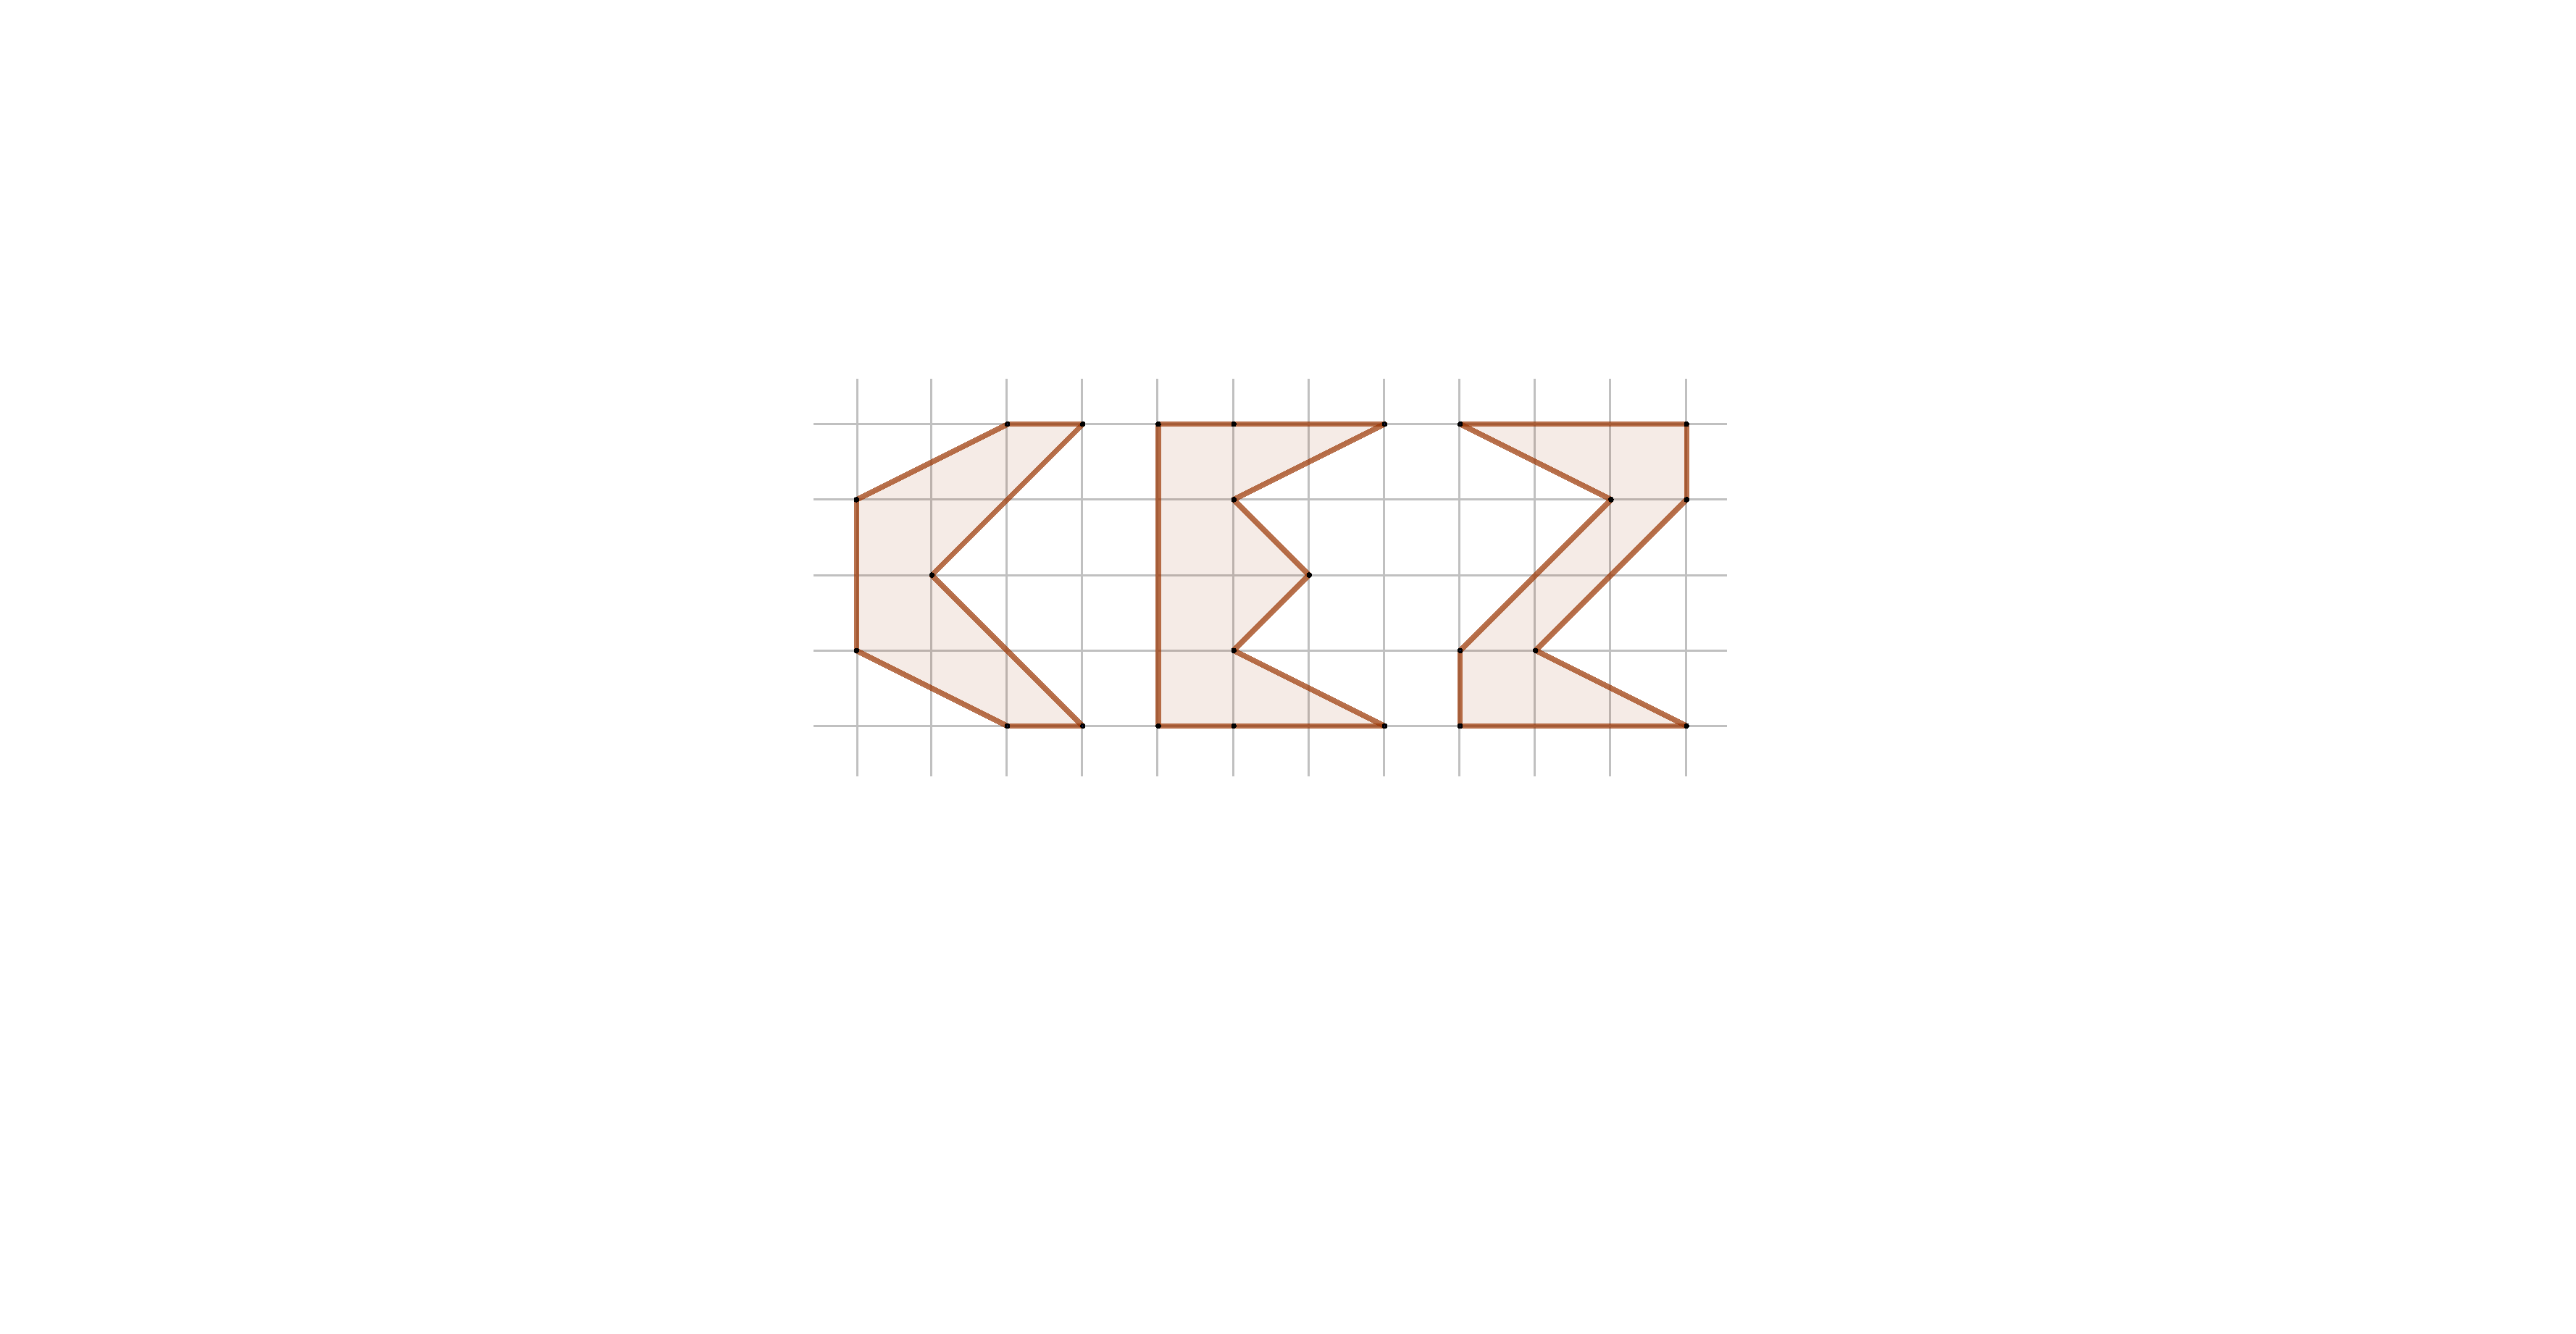
\includegraphics[width=0.6\textwidth]{úlohy/8/ctversit/11}

    \end{minipage}

    \item
    \begin{minipage}[t]{\linewidth}
        \begin{quote}
            Vypište všechny tvary, které jsou osově souměrné podle libovolné osy.
            Určete také součet obsahů tvarů C, H, F a G\@.
        \end{quote}
        \centering
        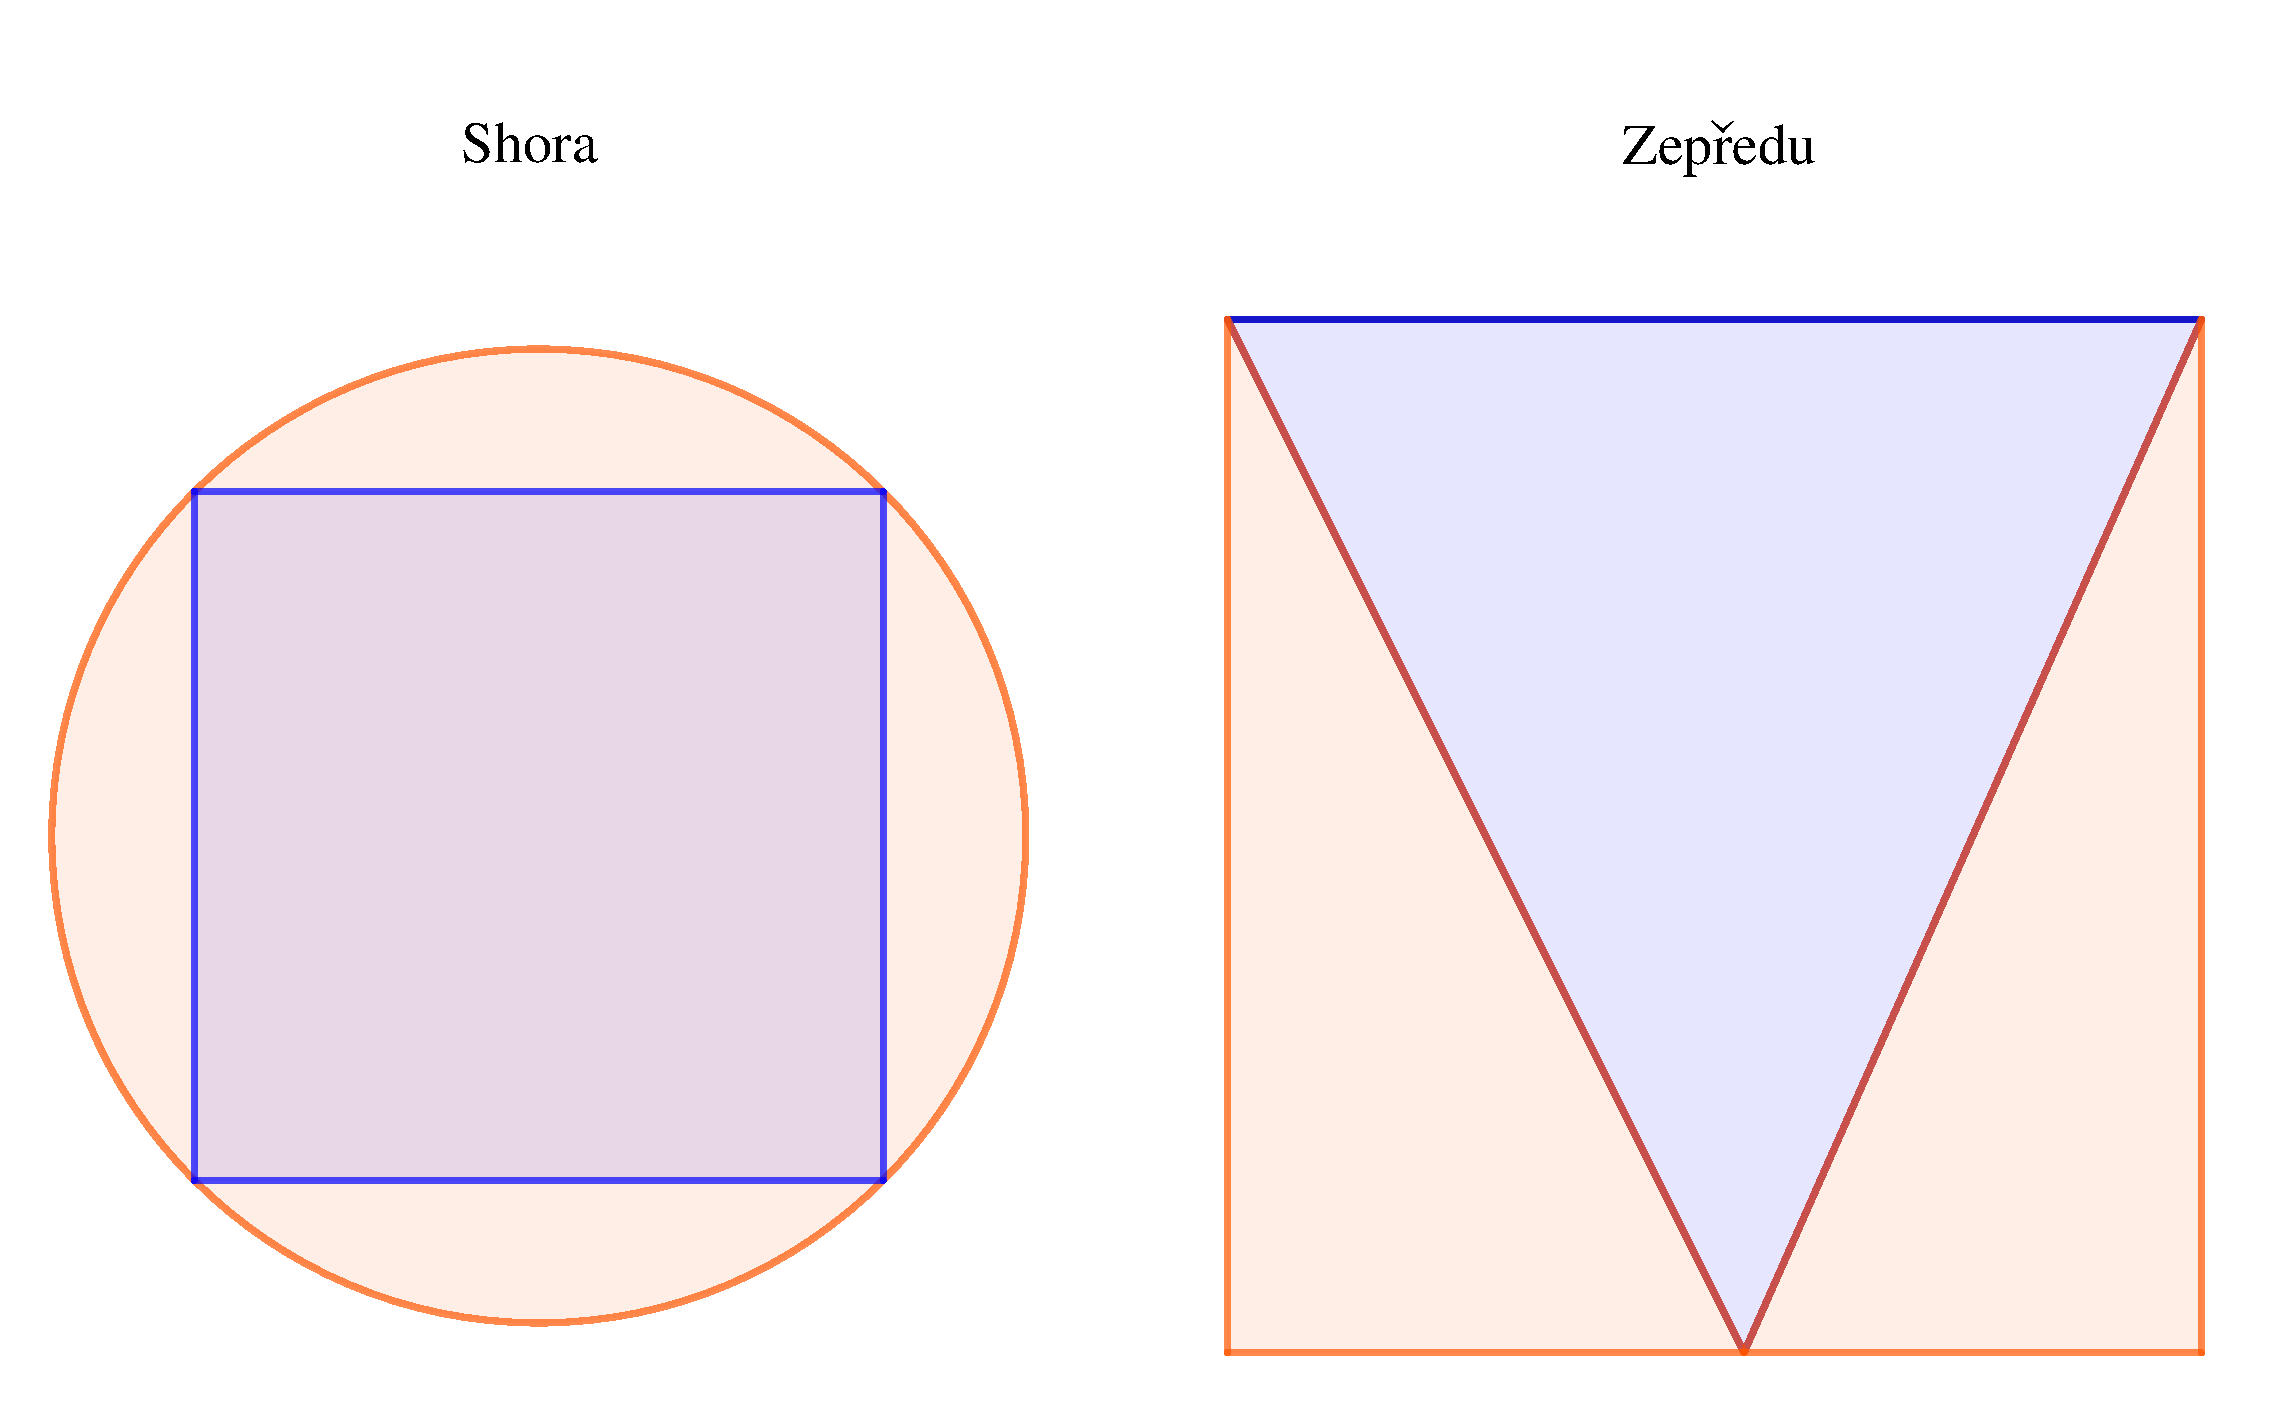
\includegraphics[width=0.7\textwidth]{úlohy/8/ctversit/12}

    \end{minipage}
\end{enumerate}

\newpage

\paragraph{Řešení}
\begin{enumerate}
    \item
    \begin{quote}
        Obsah $\triangle\text{DEF} = 7,5\,\text{cm}^2$, $\triangle\text{GCH} = 6\,\text{cm}^2$ a $\rectangle\text{ABCD} = 50\,\text{cm}^2$
    \end{quote}

    \item
    \begin{quote}
        Obsah $\text{A} = 20\,\text{cm}^2$, $\text{B} = 21\,\text{cm}^2$
    \end{quote}

    \item
    \begin{quote}
        Ano, ne, ano
    \end{quote}

    \item
    \begin{quote}
        Oba mají stejný obsah, rozdíl je tedy $0\,\text{cm}^2$.
        Tvar A má obvod delší o 2 cm.
    \end{quote}

    \item
    \begin{quote}
        Obsah $\text{A} = 5\,\text{cm}^2$, $\text{B} = 2\,\text{cm}^2$, $\text{C} = 6\,\text{cm}^2$
    \end{quote}

    \item
    \begin{quote}
        Pouze tvar A\@.
    \end{quote}

    \item
    \begin{quote}
        Obsah $\text{A} = 18\,\text{cm}^2$, $\text{B} = 18\,\text{cm}^2$, $\text{C} = 19\,\text{cm}^2$.
        Největší obsah má tvar C\@.
    \end{quote}

    \item
    \begin{quote}
        Obsah $\text{A} = 72\,\text{cm}^2$, $\text{B} = 80\,\text{cm}^2$, $\text{C} = 28\,\text{cm}^2$.
    \end{quote}

    \item
    \begin{quote}
        Oba tvary mají stejný obvod, rozdíl je tedy 0 cm.
        Obsah tvaru A je větší o $2\,\text{cm}^2$.
    \end{quote}

    \item
    \begin{quote}
        Obsah $\text{A} = 15,5\,\text{cm}^2$, $\text{B} = 8\,\text{cm}^2$, $\text{C} = 15\,\text{cm}^2$
    \end{quote}

    \item
    \begin{quote}
        Součet obsahů je $25\,\text{cm}^2$.
        Obvod písmene Z je větší než obvod písmene C\@.
    \end{quote}

    \item
    \begin{quote}
        Tvary A, B, D, E, G a I jsou souměrné podle aspoň 1 osy.
        Součet obsahů je $15\,\text{cm}^2$
    \end{quote}

\end{enumerate}

\newpage

\subsubsection{Obvod, obsah a délky}

\paragraph{Úlohy}
\begin{enumerate}
    \item
    \begin{minipage}[t]{\linewidth}
        \begin{quote}
            $\triangle$ABC je rovnostranný a $\triangle$ABD je rovnoramenný. $\lvert \text{BD} \rvert = 4\,\text{cm}$.
            Obvod $\triangle$ABD je 15 cm.
            Jaký je obvod tvaru ADBC?
        \end{quote}
        \centering
        \includegraphics[width=0.4\textwidth]{úlohy/8/obobde/1}

    \end{minipage}

    \item
    \begin{minipage}[t]{\linewidth}
        \begin{quote}
            $\triangle$ABD a $\triangle$ABE jsou rovnoramenné. $\lvert \text{AB} \rvert = 4\,\text{cm}$. $\lvert \text{AD} \rvert = 3\,\text{cm}$.
            Obvod $\triangle$ABE je 2krát delší než obvod $\triangle$ABD. Jaký je obvod tvaru ADBE?
        \end{quote}
        \centering
        \includegraphics[width=0.5\textwidth]{úlohy/8/obobde/2}

    \end{minipage}

    \item
    \begin{minipage}[t]{\linewidth}
        \begin{quote}
            $\triangle{\text{A}}_{1}$ a $\triangle{\text{A}}_{1}$ jsou navzájem shodné. $\triangle{\text{A}}_{1}$, $\triangle{\text{A}}_{1}$, $\triangle{\text{B}}$, $\triangle{\text{D}}$ jsou rovnostranné. $\triangle{\text{C}}$ je rovnoramenný.\             Obvod $\triangle{\text{A}}_{1}$ je 18 cm.
            Obvod $\triangle$D je o 3 cm delší než obvod $\triangle{\text{A}}_{1}$.
            Určete obvod $\triangle$C.
        \end{quote}
        \centering
        \includegraphics[width=0.45\textwidth]{úlohy/8/obobde/3}

    \end{minipage}

    \item
    \begin{minipage}[t]{\linewidth}
        \begin{quote}
            Z provázku byl sestrojen čtverec tak, že byl natažen po obvodu.
            Jeho obsah je $49\,\text{cm}^{2}$.
            Poté byl tento provázek rozmotán, a byl z něj vytvořen obdélník o obsahu $45\,\text{cm}^{2}$.
            Jaké jsou délky jeho stran?
            (Obrázek je pouze ilustrační)
        \end{quote}
        \centering
        \includegraphics[width=0.6\textwidth]{úlohy/8/obobde/4}

    \end{minipage}

    \item
    \begin{minipage}[t]{\linewidth}
        \begin{quote}
            Tvar vlevo má obvod 182 cm.
            Skládá se z malých a velkých čtverců.\ 4 malé čtverce se vejdou do jednoho velkého.
            Určete obvody tvaru uprostřed a vpravo.
        \end{quote}
        \centering
        \includegraphics[width=0.8\textwidth]{úlohy/8/obobde/5}

    \end{minipage}

    \item
    \begin{minipage}[t]{\linewidth}
        \begin{quote}
            Obvod malého modrého obdélníku je 72 cm.
            Jeho delší strana je 2krát delší než jeho kratší strana.
            Tvar vpravo je čtverec.
            Určete obsah prostředního tvaru.
        \end{quote}
        \centering
        \includegraphics[width=0.7\textwidth]{úlohy/8/obobde/6}

    \end{minipage}

    \item
    \begin{minipage}[t]{\linewidth}
        \begin{quote}
            Obvod $\rectangle$A je 34 cm.
            Obsah $\rectangle$B je $35\,\text{cm}^{2}$.
            Jaké jsou délky stran $\rectangle$A?
        \end{quote}
        \centering
        \includegraphics[width=0.7\textwidth]{úlohy/8/obobde/7}

    \end{minipage}

    \item
    \begin{minipage}[t]{\linewidth}
        \begin{quote}
            Zelené $\triangle$ jsou rovnostranné a pravoúhlé.
            Obvod tvaru A je 77 cm, obvod tvaru B je 82 cm.
            Jaká je délka základny zeleného $\triangle$?
        \end{quote}
        \centering
        \includegraphics[width=0.7\textwidth]{úlohy/8/obobde/8}

    \end{minipage}

    \item
    \begin{minipage}[t]{\linewidth}
        \begin{quote}
            Délka g je 14 cm.
            Jaký je obsah čtverce D?
        \end{quote}
        \centering
        \includegraphics[width=0.7\textwidth]{úlohy/8/obobde/9}

    \end{minipage}

    \item
    \begin{minipage}[t]{\linewidth}
        \begin{quote}
            Obsah $\square$ABCD je 64 cm.
            Obvod $\triangle$ABF je 2krát delší než obvod $\square$ABCD. Součet délek obou ramen $\triangle$ABF se rovná obvodu $\triangle$CDE. Jaký je obvod tvaru EDAFBC?
        \end{quote}
        \centering
        \includegraphics[width=0.7\textwidth]{úlohy/8/obobde/10}

    \end{minipage}
\end{enumerate}


\newpage

\paragraph{Řešení}
\begin{enumerate}
    \item
    \begin{quote}
        Obvod tvaru ADBC je 22 cm.
    \end{quote}

    \item
    \begin{quote}
        Obvod tvaru ADBE je 22 cm.
    \end{quote}

    \item
    \begin{quote}
        Obvod $\triangle$C je 31 cm.
    \end{quote}

    \item
    \begin{quote}
        Délky stran jsou 9 cm a 5 cm.
    \end{quote}

    \item
    \begin{quote}
        Obvod tvaru uprostřed je 312 cm.
        Obvod tvaru vpravo je 130 cm.
    \end{quote}

    \item
    \begin{quote}
        Obsah prostředního tvaru je $216\,\text{cm}^{2}$
    \end{quote}

    \item
    \begin{quote}
        Délky stran jsou 10 cm a 7 cm.
    \end{quote}

    \item
    \begin{quote}
        Délka základny zeleného $\triangle$ je 5 cm.
    \end{quote}

    \item
    \begin{quote}
        Obsah $\square$D je $4\,\text{cm}^{2}$
    \end{quote}

    \item
    \begin{quote}
        Obvod tvaru EDAFBC je 120 cm?
    \end{quote}
\end{enumerate}

\newpage

\subsubsection{Rekurzivní úlohy}
Úlohy zaměřené na opakování jevů.

\paragraph{Úlohy}
\begin{enumerate}
    \item
    \begin{minipage}[t]{\linewidth}
        \begin{quote}

        \end{quote}
        \centering
        \includegraphics[width=0.7\textwidth]{úlohy/8/rekur/1}
    \end{minipage}

    \item
    \begin{minipage}[t]{\linewidth}
        \begin{quote}

        \end{quote}
        \centering
        \includegraphics[width=0.6\textwidth]{úlohy/8/rekur/2}
    \end{minipage}

    \item
    \begin{minipage}[t]{\linewidth}
        \begin{quote}

        \end{quote}
        \centering
        \includegraphics[width=0.7\textwidth]{úlohy/8/rekur/3}
    \end{minipage}

    \item
    \begin{minipage}[t]{\linewidth}
        \begin{quote}

        \end{quote}
        \centering
        \includegraphics[width=0.8\textwidth]{úlohy/8/rekur/4}
    \end{minipage}

    \item
    \begin{minipage}[t]{\linewidth}
        \begin{quote}

        \end{quote}
        \centering
        \includegraphics[width=0.6\textwidth]{úlohy/8/rekur/5}
    \end{minipage}

    \item
    \begin{minipage}[t]{\linewidth}
        \begin{quote}

        \end{quote}
        \centering
        \includegraphics[width=0.5\textwidth]{úlohy/8/rekur/6}
    \end{minipage}


\end{enumerate}

\newpage

\paragraph{Řešení}
\begin{enumerate}
    \item
    \begin{quote}
        `
    \end{quote}

    \item
    \begin{quote}
        2
    \end{quote}

    \item
    \begin{quote}
        3
    \end{quote}

    \item
    \begin{quote}
        4
    \end{quote}

    \item
    \begin{quote}
        5
    \end{quote}

    \item
    \begin{quote}
        6
    \end{quote}
\end{enumerate}

\newpage

\subsection{Rýsování}
\label{subsec:rysovani}

\subsubsection{Podle bodů}

\paragraph{Úlohy}
\begin{enumerate}
    \item
    \begin{minipage}[t]{\linewidth}
        \begin{quote}
            Narýsujte $\square$ABED tak, aby v něm ležel bod C. Dále sestrojte $\triangle$DCE\@.
        \end{quote}
        \centering
        \includegraphics[width=\textwidth]{úlohy/8/rysovani/b/1}

    \end{minipage}

    \item
    \begin{minipage}[t]{\linewidth}
        \begin{quote}
            Narýsujte $\rectangle$ACDE tak, aby na $\overleftrightarrow{\text{ED}}$ ležel bod B\@.
        \end{quote}
        \centering
        \includegraphics[width=\textwidth]{úlohy/8/rysovani/b/2}

    \end{minipage}

    \item
    \begin{minipage}[t]{\linewidth}
        \begin{quote}
            Narýsujte $\square$ADEF. Bod D leží na $\overline{\text{AB}}$ a bod E leží na $\overline{\text{DC}}$. $\angle$ABD tedy musí být pravý.
        \end{quote}
        \centering
        \includegraphics[width=\textwidth]{úlohy/8/rysovani/b/3}

    \end{minipage}

    \item
    \begin{minipage}[t]{\linewidth}
        \begin{quote}
            Narýsujte $\square$BCDE tak, aby se v něm nenacházel bod A. Následovně narýsujte bod A', který je osově souměrný bodu A dle $\overline{\text{BC}}$.
            Poté sestrojte $\triangle$AA'B.
        \end{quote}
        \centering
        \includegraphics[width=\textwidth]{úlohy/8/rysovani/b/4}

    \end{minipage}

    \item
    \begin{minipage}[t]{\linewidth}
        \begin{quote}
            Narýsujte $\rectangle$ABDE tak, aby $\lvert \overline{\text{BC}} \rvert$ = $\lvert \overline{\text{CD}} \rvert$.
        \end{quote}
        \centering
        \includegraphics[width=\textwidth]{úlohy/8/rysovani/b/5}

    \end{minipage}

    \item
    \begin{minipage}[t]{\linewidth}
        \begin{quote}
            Narýsujte $\rectangle$BCDF tak, aby $\lvert \overline{\text{AB}} \rvert$ = $\lvert \overline{\text{AD}} \rvert$.
            Sestrojte všechny možnosti.
        \end{quote}
        \centering
        \includegraphics[width=\textwidth]{úlohy/8/rysovani/b/6}

    \end{minipage}
\end{enumerate}


\newpage

\paragraph{Řešení}
\begin{enumerate}
    \item
    \begin{minipage}[t]{\linewidth}
        \begin{quote}
            \phantom{text}
        \end{quote}
        \centering
        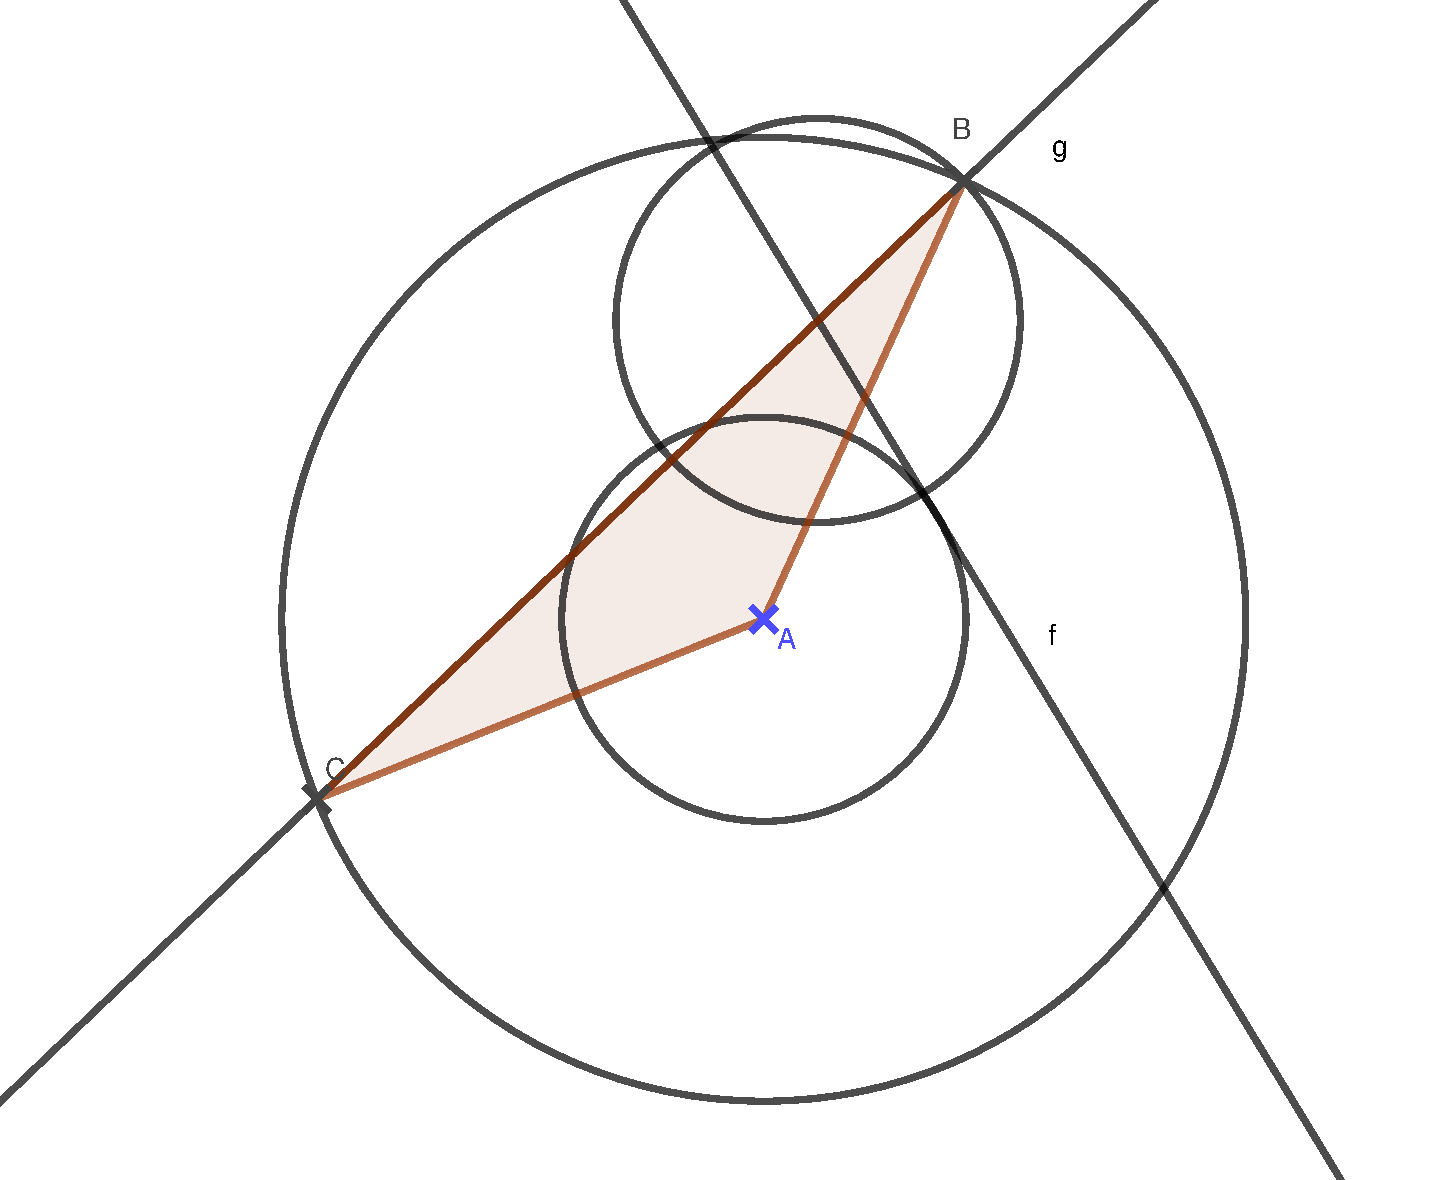
\includegraphics[width=0.5\textwidth]{úlohy/8/rysovani/b/1-v}

    \end{minipage}

    \item
    \begin{minipage}[t]{\linewidth}
        \begin{quote}
            \phantom{text}
        \end{quote}
        \centering
        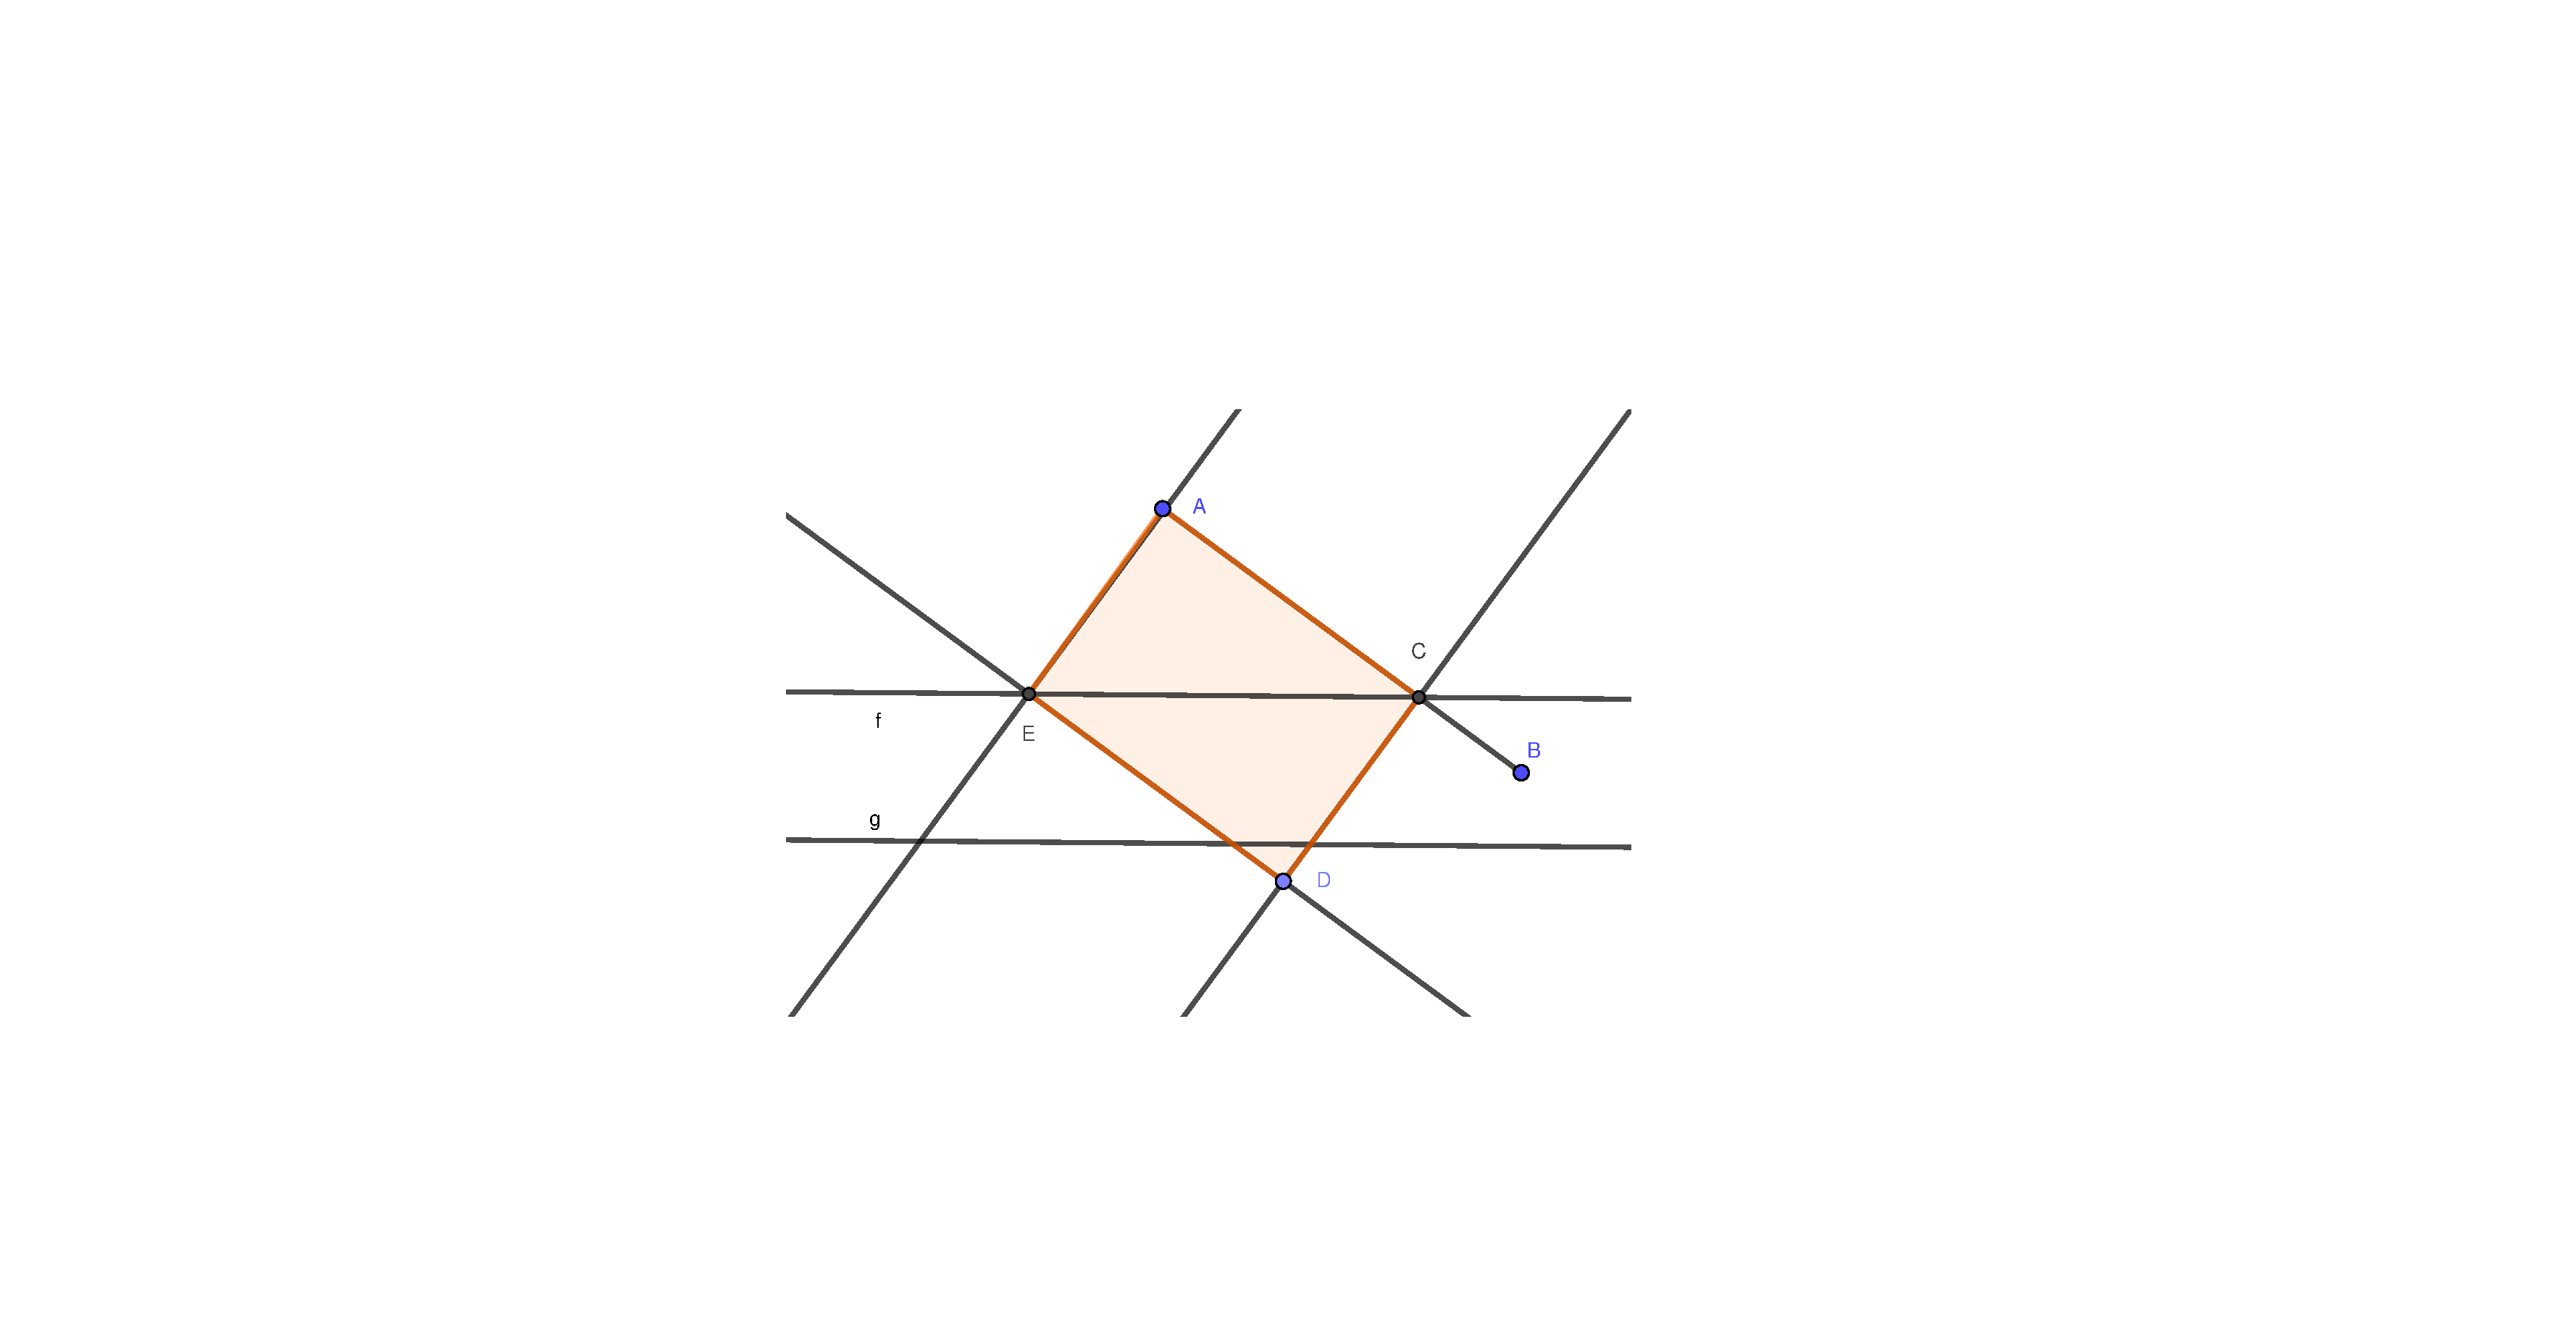
\includegraphics[width=0.7\textwidth]{úlohy/8/rysovani/b/2-v}

    \end{minipage}

    \item
    \begin{minipage}[t]{\linewidth}
        \begin{quote}
            \phantom{text}
        \end{quote}
        \centering
        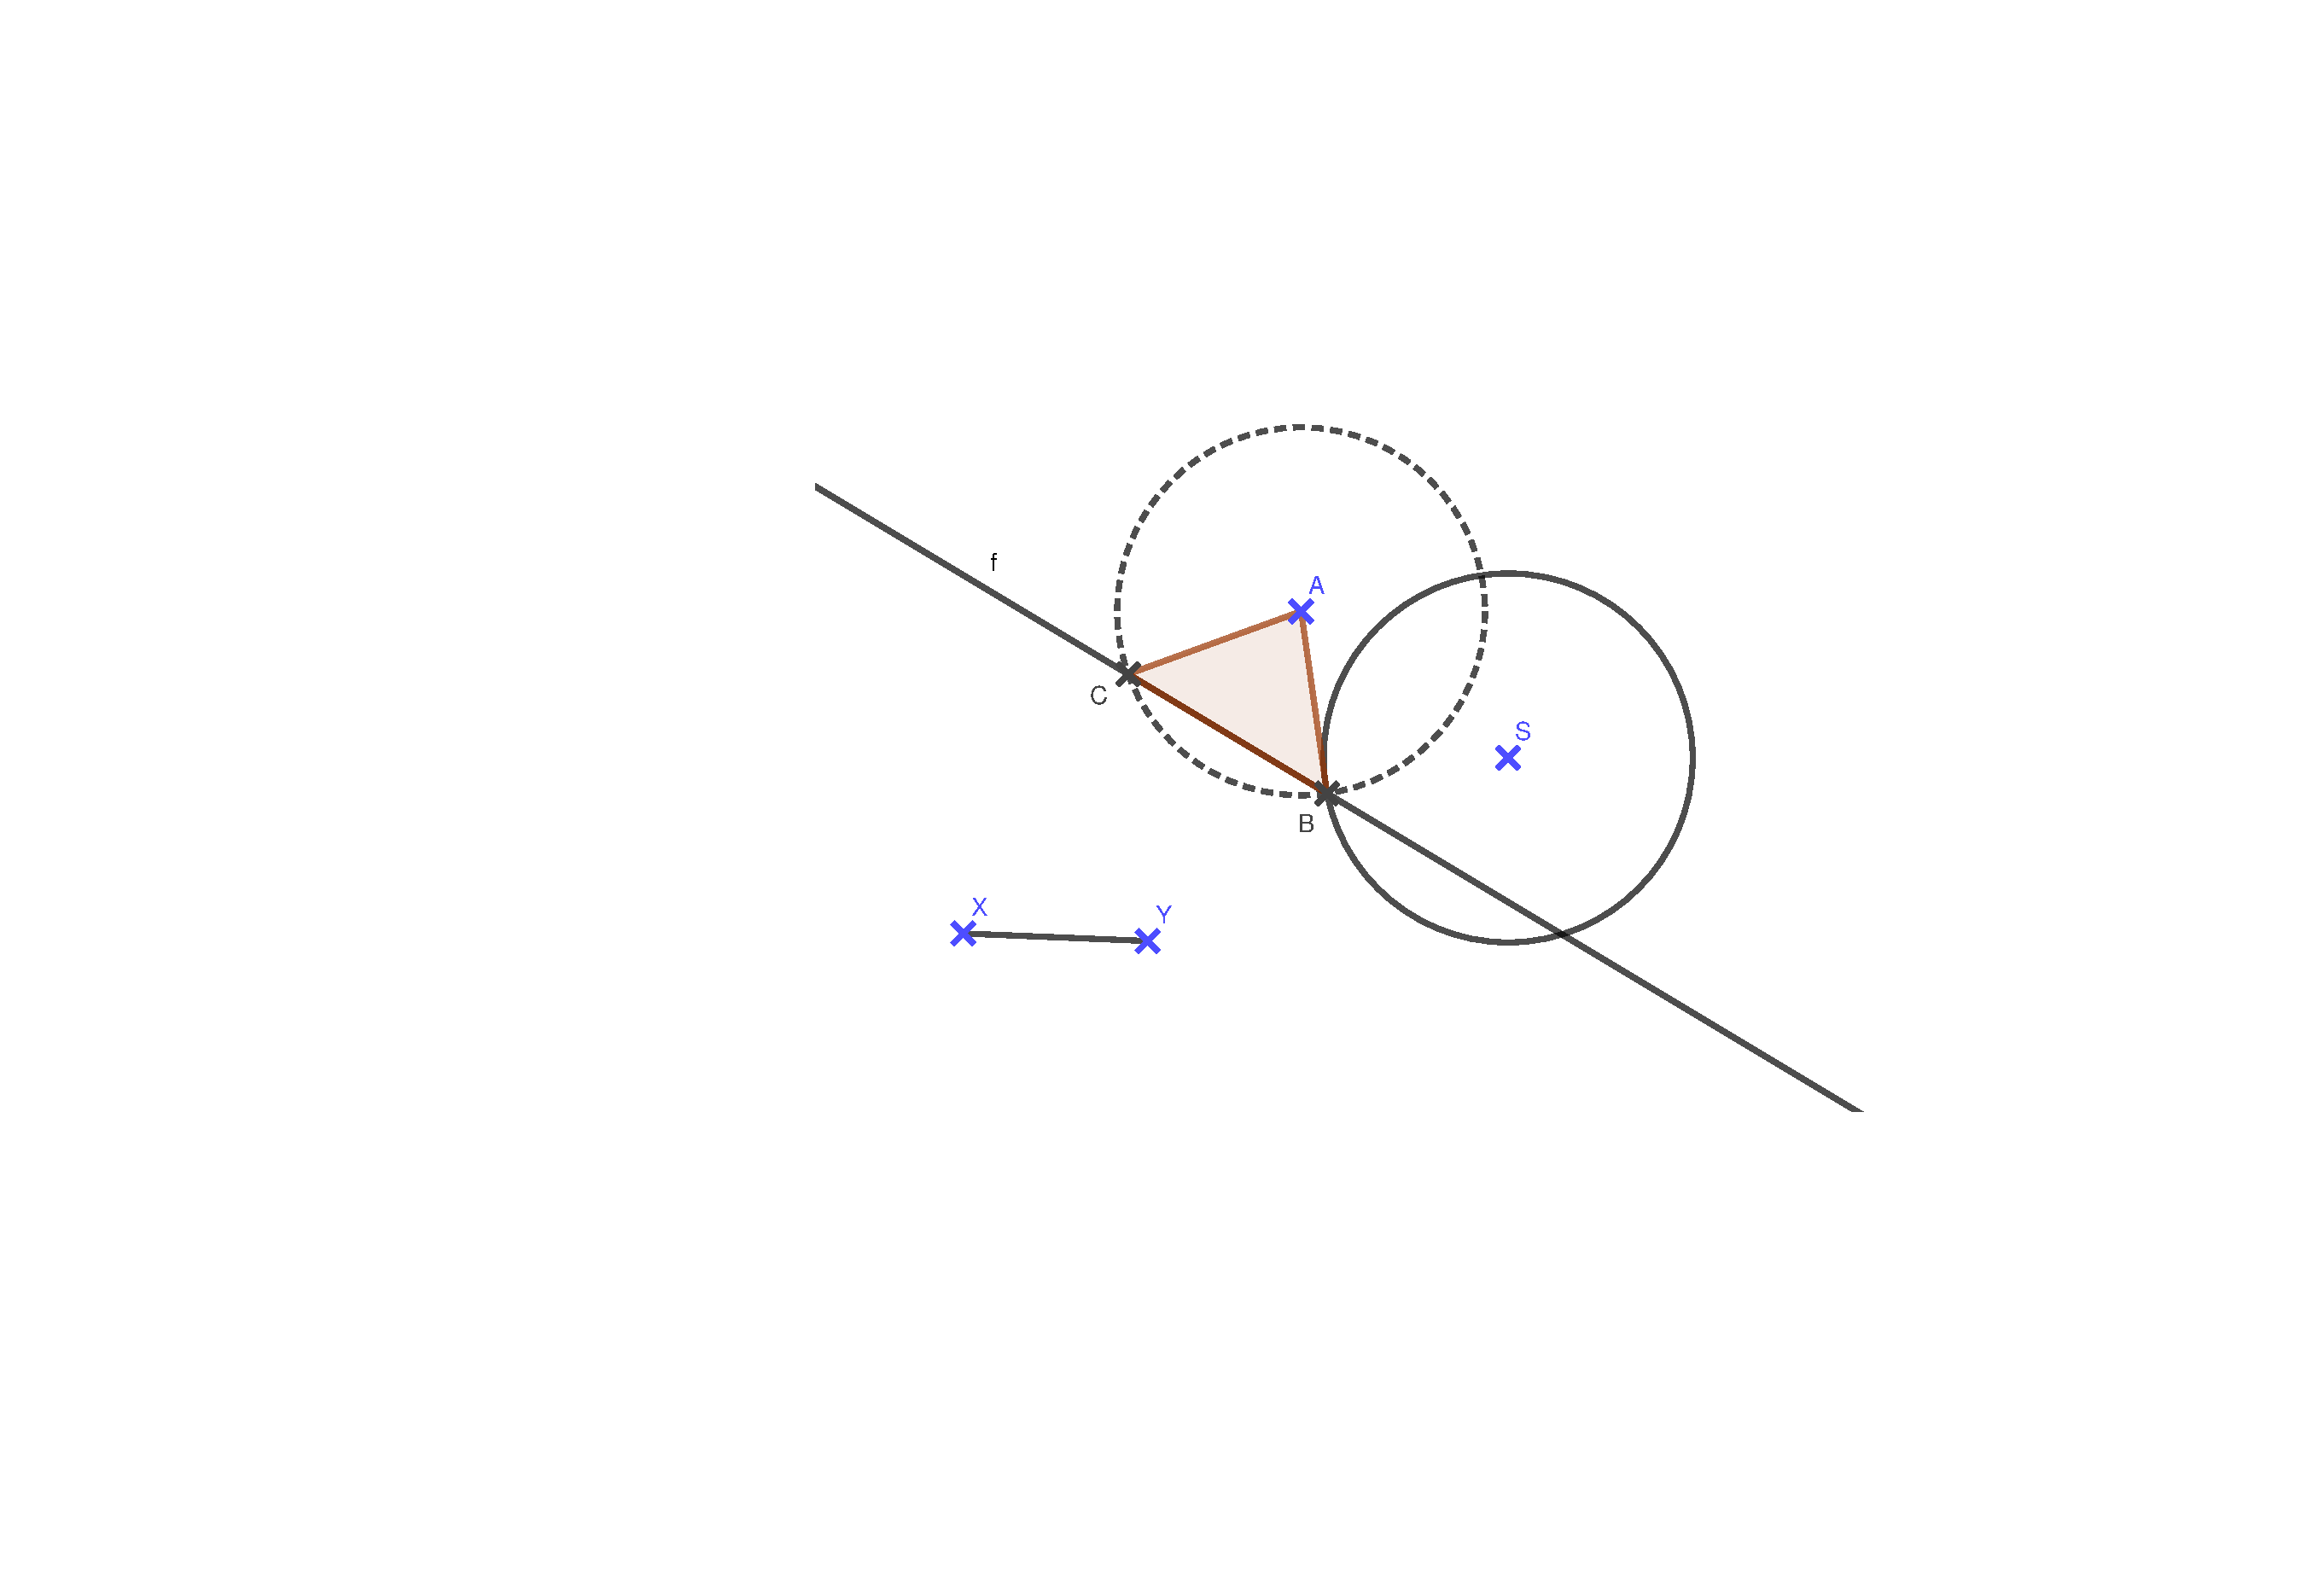
\includegraphics[width=0.8\textwidth]{úlohy/8/rysovani/b/3-v}

    \end{minipage}

    \item
    \begin{minipage}[t]{\linewidth}
        \begin{quote}
            \phantom{text}
        \end{quote}
        \centering
        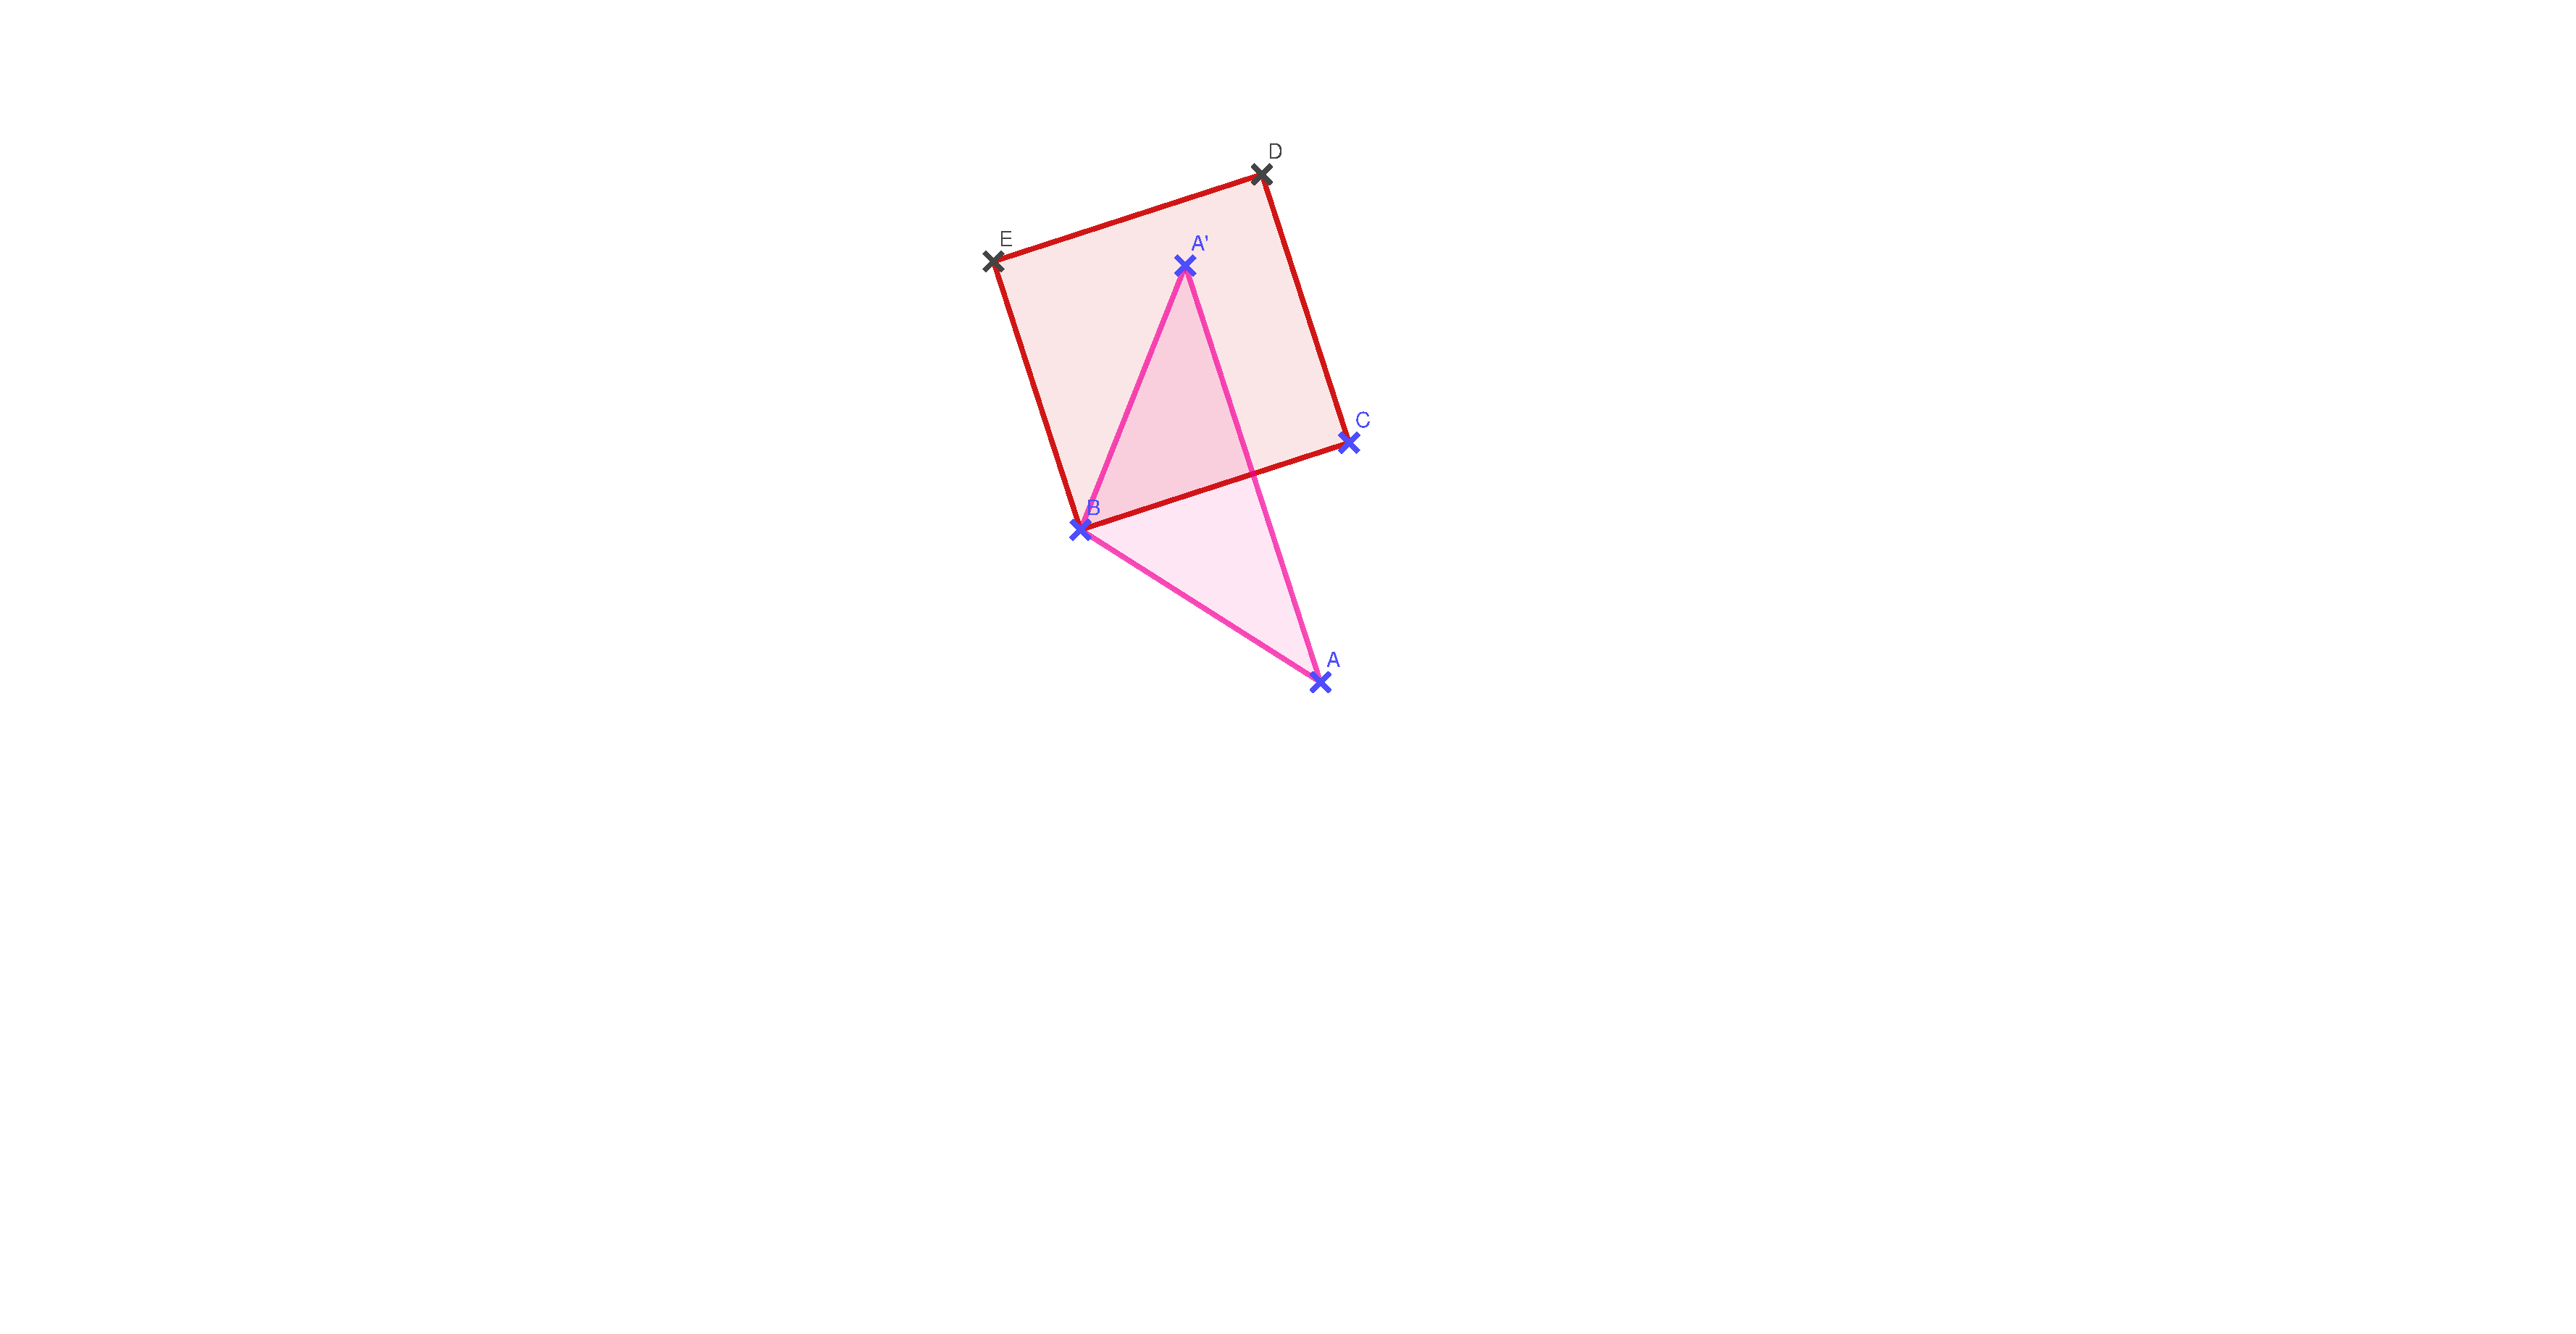
\includegraphics[width=0.7\textwidth]{úlohy/8/rysovani/b/4-v}

    \end{minipage}

    \item
    \begin{minipage}[t]{\linewidth}
        \begin{quote}
            \phantom{text}
        \end{quote}
        \centering
        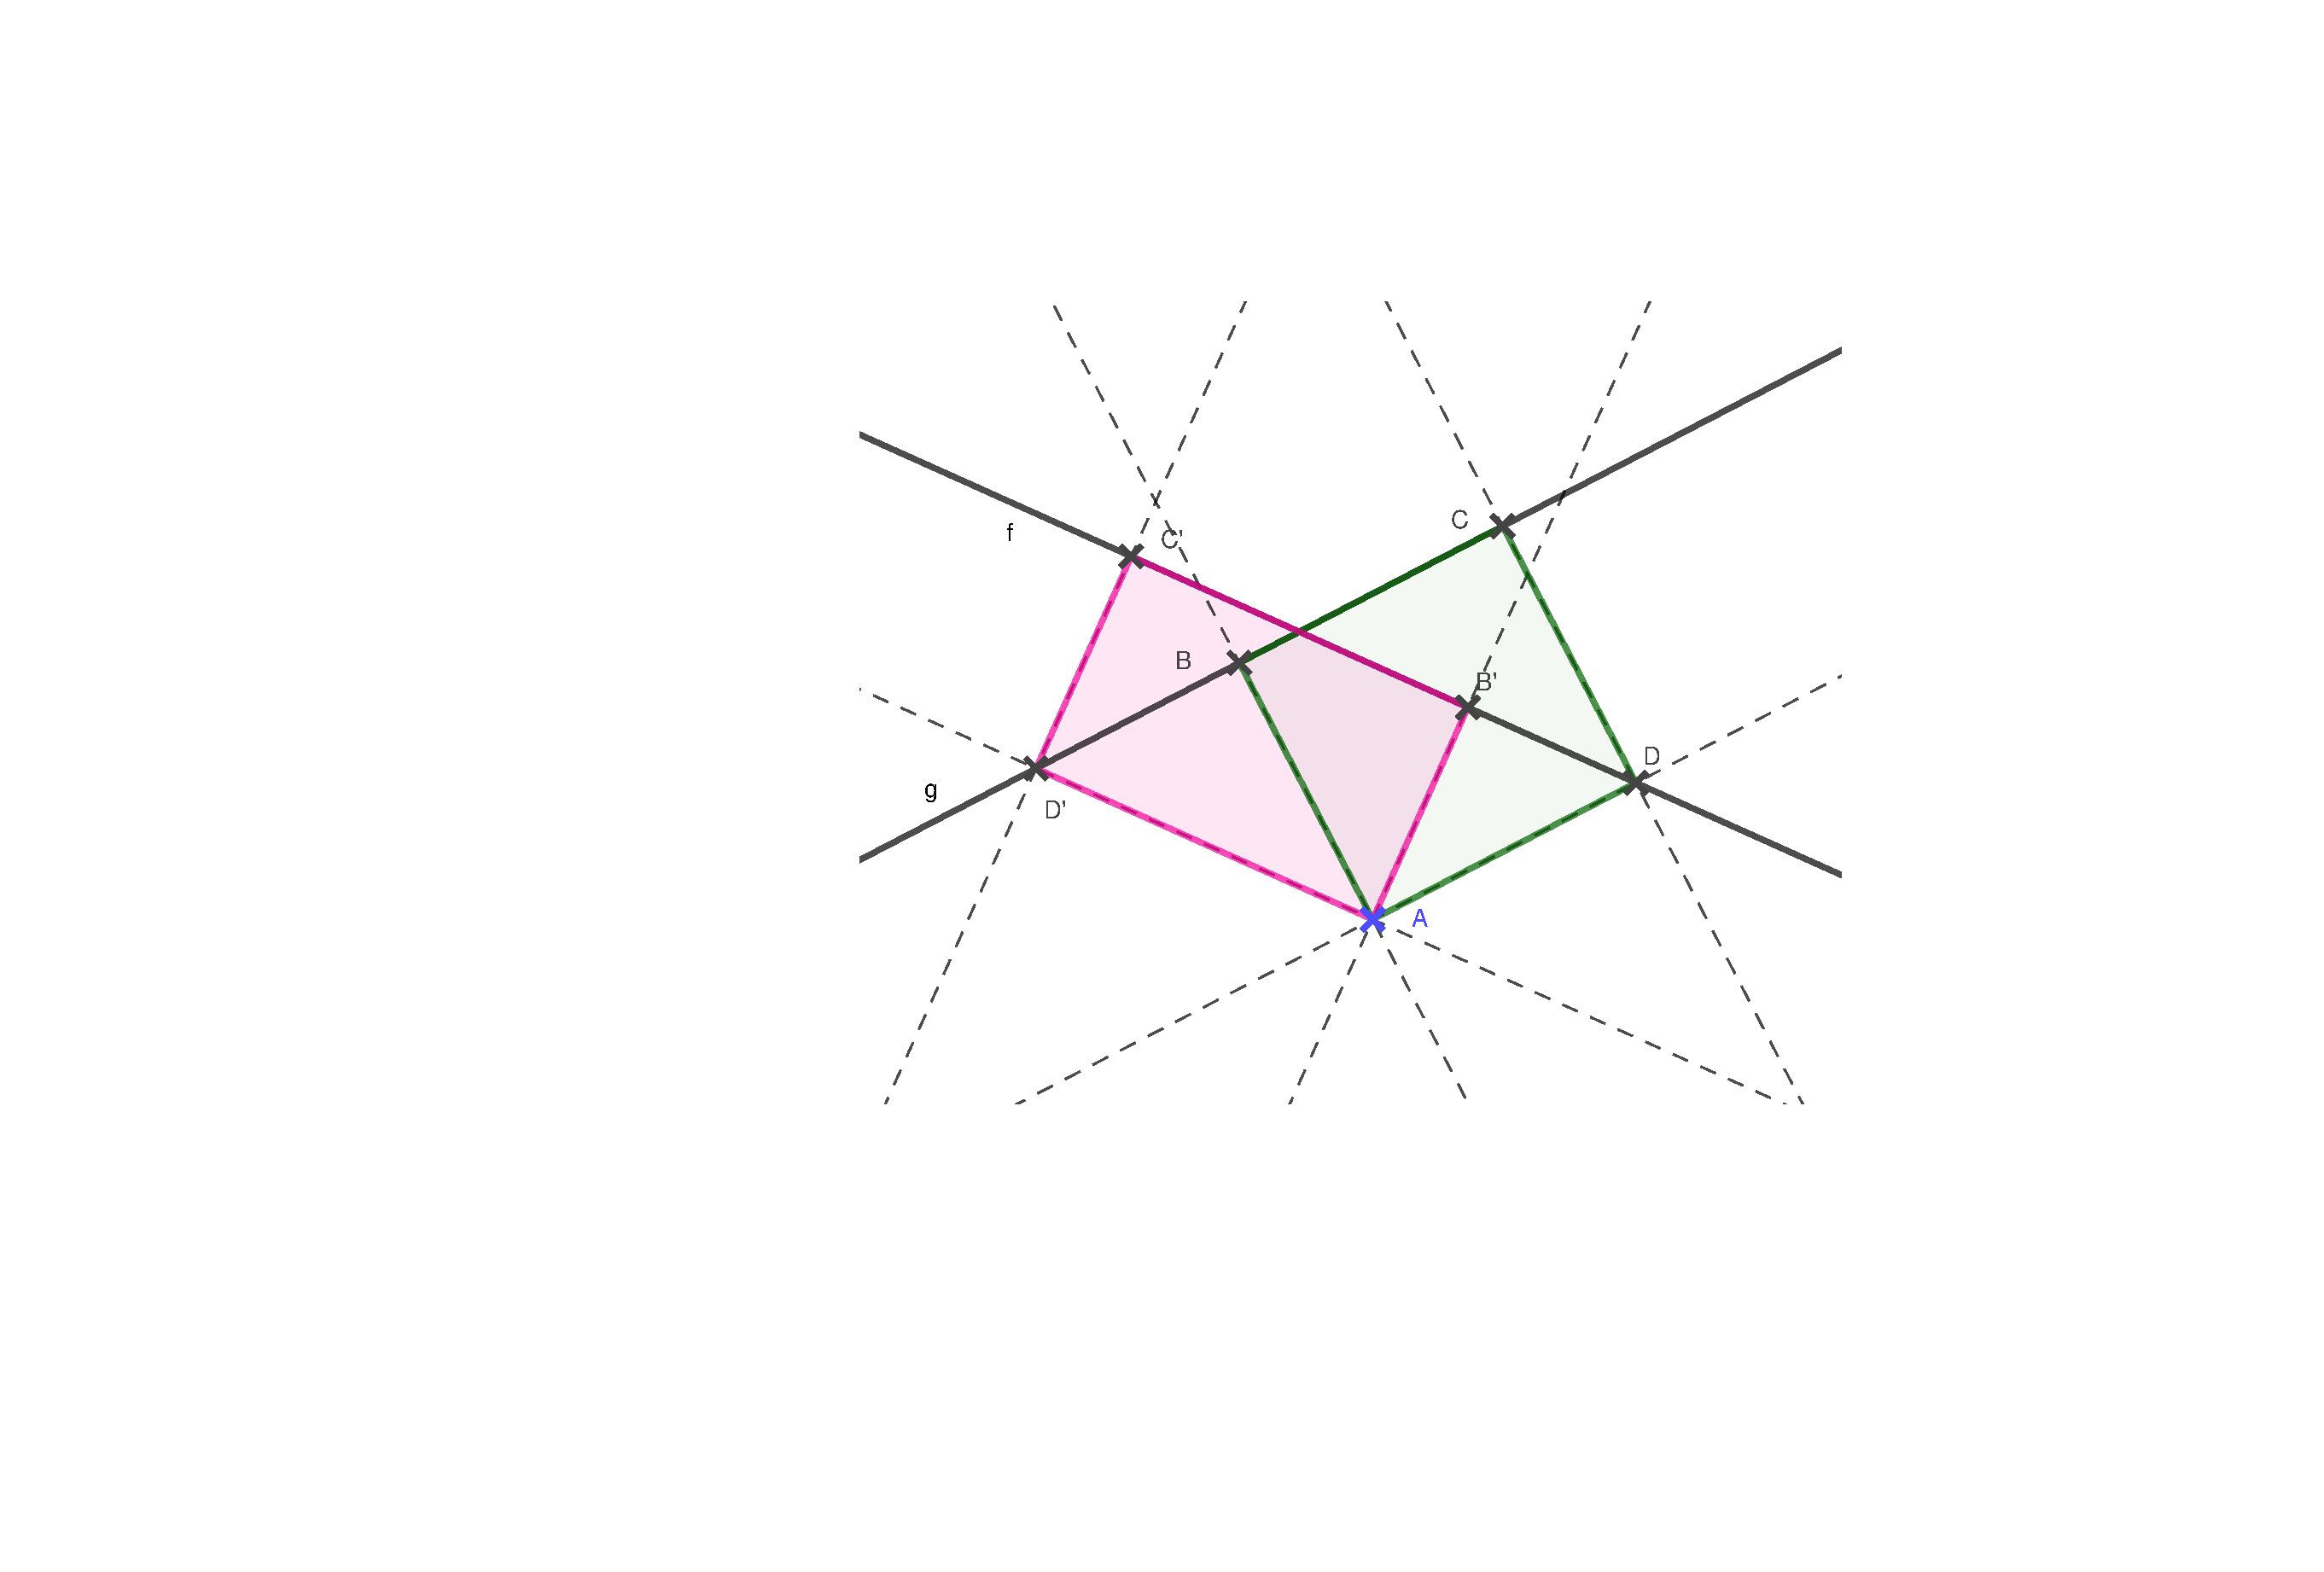
\includegraphics[width=0.6\textwidth]{úlohy/8/rysovani/b/5-v}

    \end{minipage}

    \item
    \begin{minipage}[t]{\linewidth}
        \begin{quote}
            \phantom{text}
        \end{quote}
        \centering
        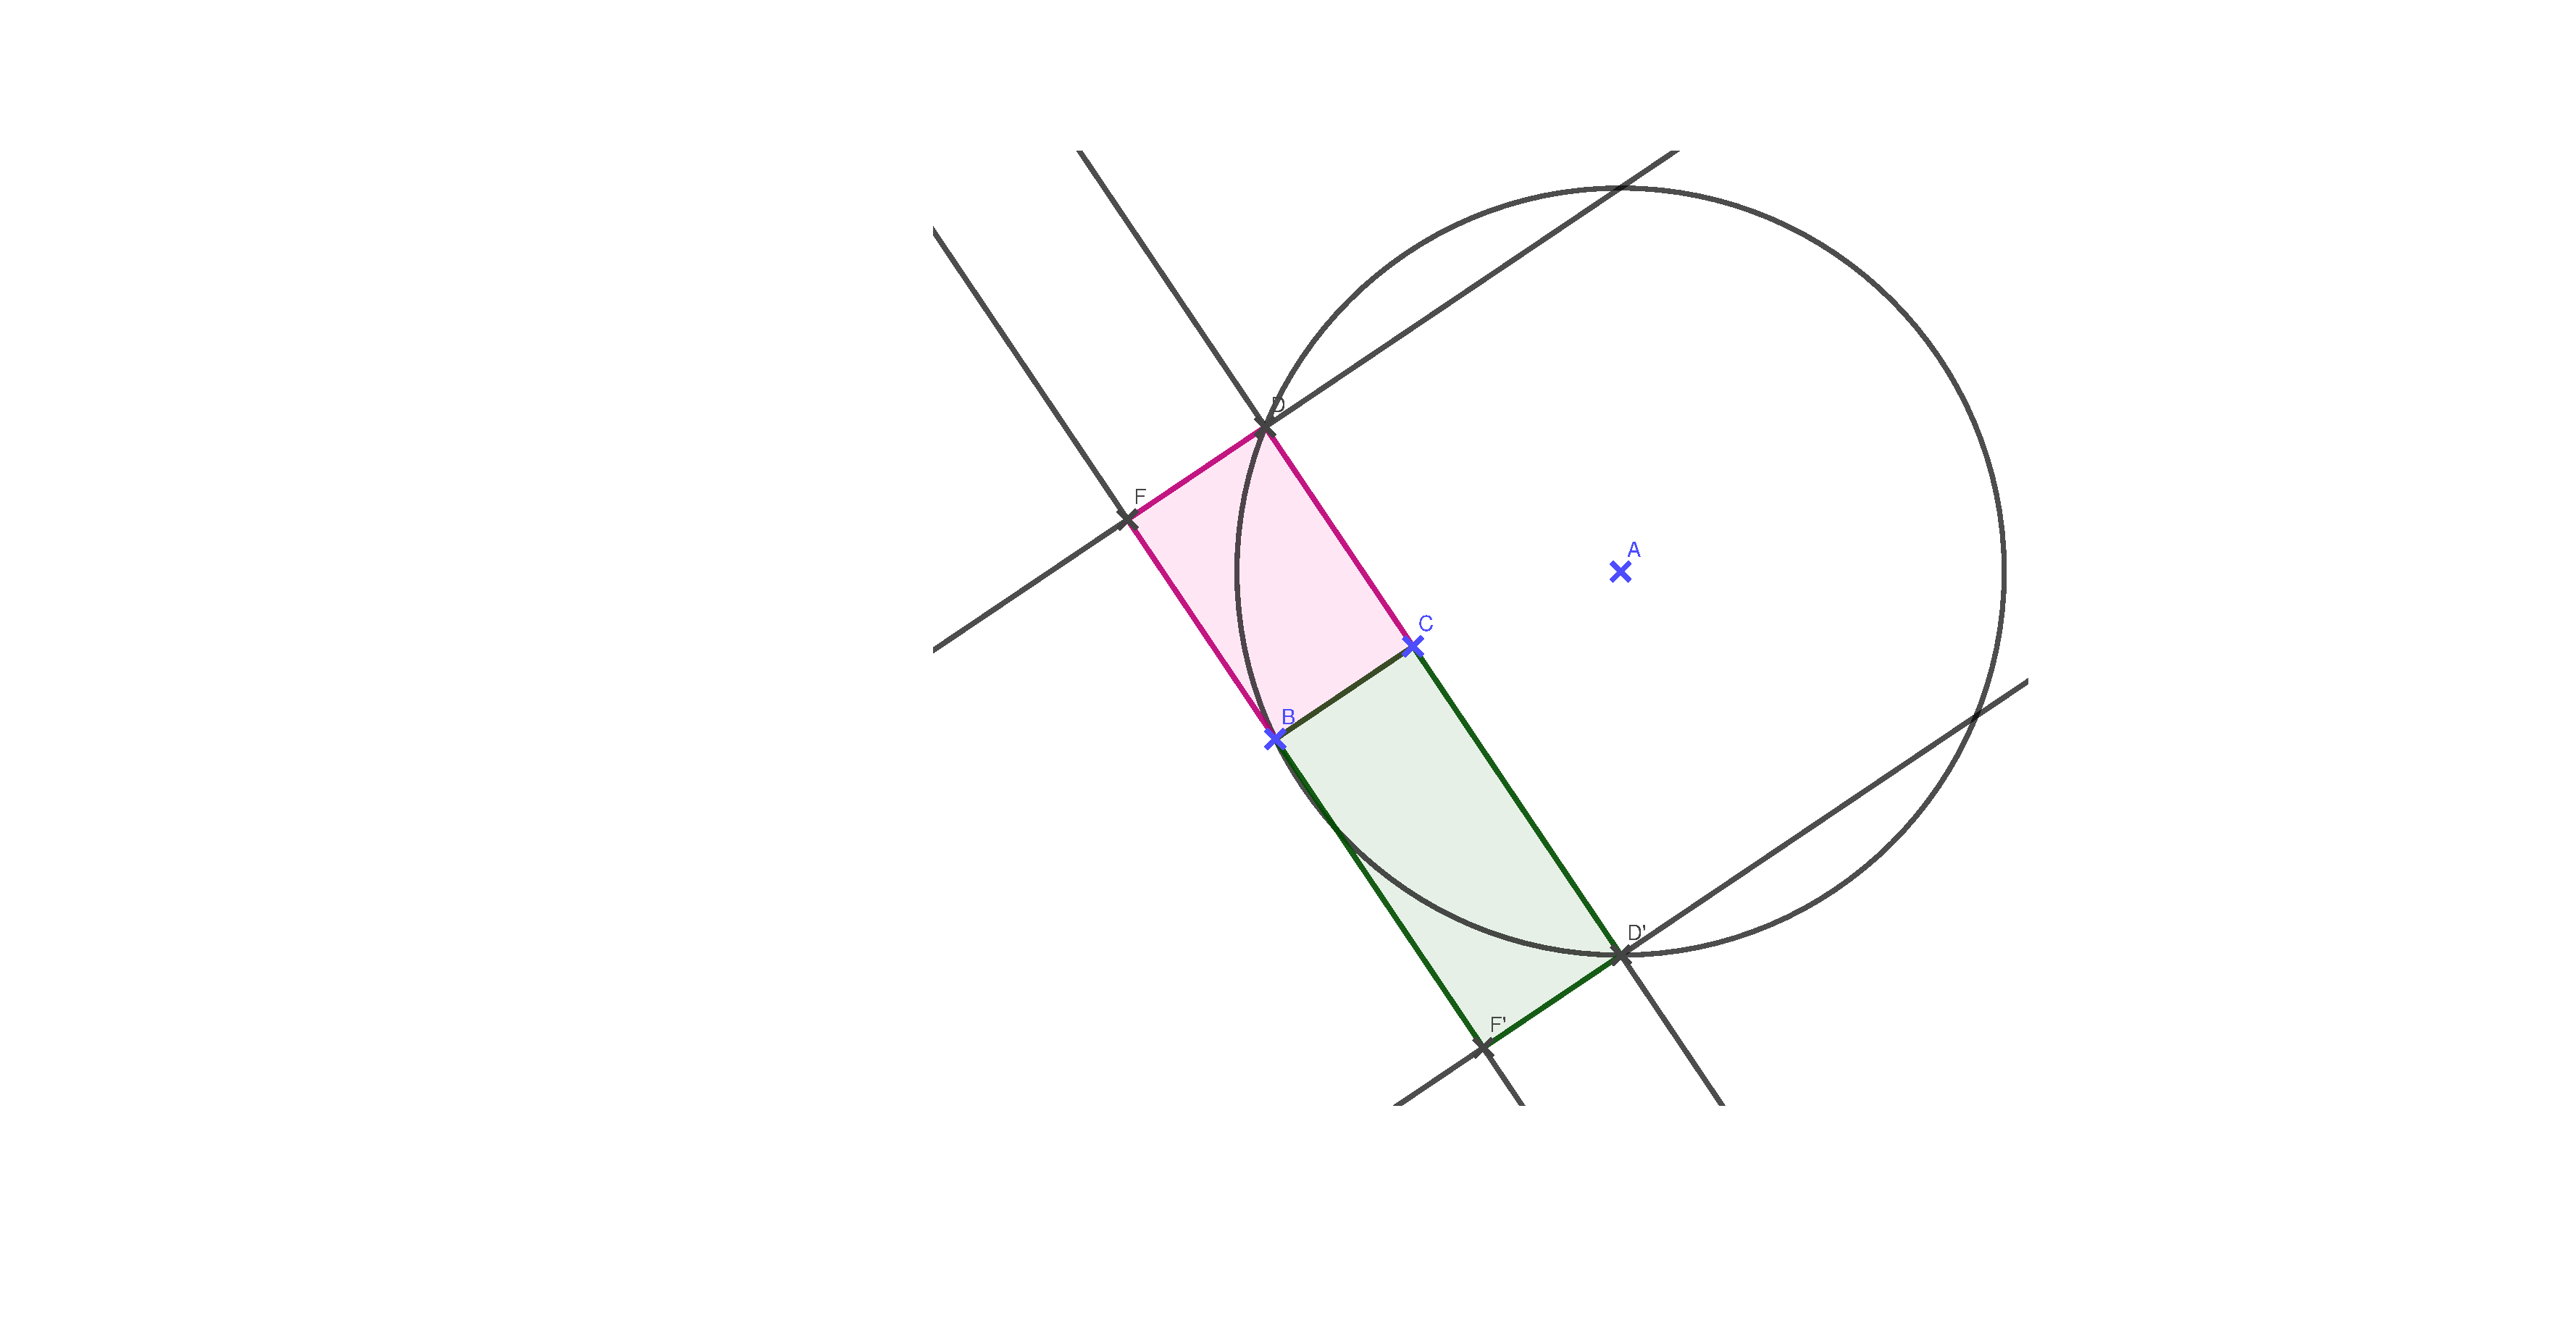
\includegraphics[width=0.6\textwidth]{úlohy/8/rysovani/b/6-v}

    \end{minipage}
\end{enumerate}

\newpage

\subsubsection{Podle bodů a čar}

\paragraph{Úlohy}
\begin{enumerate}
    \item
    \begin{minipage}[t]{\linewidth}
        \begin{quote}
            Narýsujte rovnoramenný $\triangle$ABC, jehož základna leží na $\overleftrightarrow{\text{g}}$.
            Platí, že $\lvert \overleftrightarrow{\text{f}} \text{A} \rvert = \lvert \overleftrightarrow{\text{f}} \text{B} \rvert$.
        \end{quote}
        \centering
        \includegraphics[width=0.8\textwidth]{úlohy/8/rysovani/bp/1}

    \end{minipage}

    \item
    \begin{minipage}[t]{\linewidth}
        \begin{quote}
            Narýsujte $\rectangle$ABCD tak, aby bod C ležel na $\overleftrightarrow{\text{g}}$ a bod D na $\overleftrightarrow{\text{f}}$
        \end{quote}
        \centering
        \includegraphics[width=0.8\textwidth]{úlohy/8/rysovani/bp/2}

    \end{minipage}

    \item
    \begin{minipage}[t]{\linewidth}
        \begin{quote}
            Narýsujte rovnoramenný $\triangle$ABC, jehož základna leží na $\overleftrightarrow{\text{f}}$.
            Platí $\lvert \overline{\text{XY}} \rvert = \lvert \overline{\text{SB}} \rvert$.
        \end{quote}
        \centering
        \includegraphics[width=0.6\textwidth]{úlohy/8/rysovani/bp/3}

    \end{minipage}

    \item
    \begin{minipage}[t]{\linewidth}
        \begin{quote}
            Narýsujte rovnoramenný $\triangle$ABC, jehož základna leží na $\overleftrightarrow{\text{f}}$.
            Následně vytvořte rovnostranný $\triangle{\text{CDE}}$ tak, aby $\overline{\text{AB}} \perp \overline{\text{CD}}$ a bod E nenáležel $\triangle$ABC\@.
        \end{quote}
        \centering
        \includegraphics[width=0.7\textwidth]{úlohy/8/rysovani/bp/4}

    \end{minipage}

    \item
    \begin{minipage}[t]{\linewidth}
        \begin{quote}
            Sestrojte $\square$ABCD tak, aby bod D ležel na jedné z přímek a aby strana B byla kolmá na druhou.
            Narýsujte všechny možnosti.
        \end{quote}
        \centering
        \includegraphics[width=0.7\textwidth]{úlohy/8/rysovani/bp/5}

    \end{minipage}

    \item
    \begin{minipage}[t]{\linewidth}
        \begin{quote}
            Narýsujte $\rectangle$ABCD tak, aby strana b ležela na $\overrightarrow{\text{XY}}$, $\lvert \overrightarrow{\text{XY}} \text{A} \rvert = \lvert \text{AZ} \rvert$ a $\lvert \text{BC} \rvert = \lvert \text{BZ} \rvert$.
        \end{quote}
        \centering
        \includegraphics[width=0.8\textwidth]{úlohy/8/rysovani/bp/6}

    \end{minipage}

    \item
    \begin{minipage}[t]{\linewidth}
        \begin{quote}
            Narýsujte $\rectangle$ABCD tak, aby středem $\overline{\text{YZ}}$ byl zároveň středem $\overline{\text{BC}}$.
        \end{quote}
        \centering
        \includegraphics[width=0.8\textwidth]{úlohy/8/rysovani/bp/7}

    \end{minipage}

    \item
    \begin{minipage}[t]{\linewidth}
        \begin{quote}
            Narýsujte rovnoramenný $\triangle$ABC tak, aby bod B ležel na $\overline{\text{ZY}}$, $\lvert \text{SB} \rvert = \lvert \text{SA} \rvert$.
            Základnou je strana BC\@.
        \end{quote}
        \centering
        \includegraphics[width=0.8\textwidth]{úlohy/8/rysovani/bp/8}

    \end{minipage}

    \item
    \begin{minipage}[t]{\linewidth}
        \begin{quote}
            Narýsujte pravoúhlý $\triangle$ABC aby bod B ležel na $\overline{\text{ZY}}$ a strana AC byla jeho nejdelší stranou.

            Dále narýsujte $\triangle$ACD jehož pravý úhel leží u bodu A aby platilo $\lvert \text{AB} \rvert = \lvert \text{AD} \rvert$.

            Jako poslední narýsujte rovnostranný $\triangle$CED tak, aby $\lvert \text{ED} \rvert > \lvert \text{EA} \rvert$.
        \end{quote}
        \centering
        \includegraphics[width=0.8\textwidth]{úlohy/8/rysovani/bp/9}

    \end{minipage}

    \item
    \begin{minipage}[t]{\linewidth}
        \begin{quote}
            Narýsujte $\square$ABCD kterým prochází $\overleftrightarrow{\text{f}}$.

            Dále sestrojte $\triangle$EDF tak, aby se bod E nacházel na průsečíku $\overleftrightarrow{\text{f}}$ a $\overleftrightarrow{\text{CD}}$, bod F se nacházel na $\overleftrightarrow{\text{AC}}$ a $\lvert \text{AF} \rvert = \lvert \text{AC}$
        \end{quote}
        \centering
        \includegraphics[width=0.8\textwidth]{úlohy/8/rysovani/bp/10}

    \end{minipage}

    \item
    \begin{minipage}[t]{\linewidth}
        \begin{quote}
            Narýsujte $\triangle$ABH aby $\lvert \text{BH} \rvert = \lvert \text{ED} \rvert$, $\lvert \text{AH} \rvert < \lvert \text{EF} \rvert$ a aby se bod H nacházel na lomené čáře CDEFG\@.
        \end{quote}
        \centering
        \includegraphics[width=0.8\textwidth]{úlohy/8/rysovani/bp/11}

    \end{minipage}
\end{enumerate}


\newpage

\paragraph{Řešení}
\begin{enumerate}
    \item
    \begin{minipage}[t]{\linewidth}
        \begin{quote}
            \phantom{text}
        \end{quote}
        \centering
        \includegraphics[width=0.6\textwidth]{úlohy/8/rysovani/bp/1-v}

    \end{minipage}

    \item
    \begin{minipage}[t]{\linewidth}
        \begin{quote}
            \phantom{text}
        \end{quote}
        \centering
        \includegraphics[width=0.6\textwidth]{úlohy/8/rysovani/bp/2-v}

    \end{minipage}

    \item
    \begin{minipage}[t]{\linewidth}
        \begin{quote}
            \phantom{text}
        \end{quote}
        \centering
        \includegraphics[width=0.6\textwidth]{úlohy/8/rysovani/bp/3-v}

    \end{minipage}

    \item
    \begin{minipage}[t]{\linewidth}
        \begin{quote}
            \phantom{text}
        \end{quote}
        \centering
        \includegraphics[width=0.6\textwidth]{úlohy/8/rysovani/bp/4-v}

    \end{minipage}

    \item
    \begin{minipage}[t]{\linewidth}
        \begin{quote}
            \phantom{text}
        \end{quote}
        \centering
        \includegraphics[width=0.6\textwidth]{úlohy/8/rysovani/bp/5-v}

    \end{minipage}

    \item
    \begin{minipage}[t]{\linewidth}
        \begin{quote}
            \phantom{text}
        \end{quote}
        \centering
        \includegraphics[width=0.6\textwidth]{úlohy/8/rysovani/bp/6-v}

    \end{minipage}

    \item
    \begin{minipage}[t]{\linewidth}
        \begin{quote}
            \phantom{text}
        \end{quote}
        \centering
        \includegraphics[width=0.6\textwidth]{úlohy/8/rysovani/bp/7-v}

    \end{minipage}

    \item
    \begin{minipage}[t]{\linewidth}
        \begin{quote}
            \phantom{text}
        \end{quote}
        \centering
        \includegraphics[width=0.6\textwidth]{úlohy/8/rysovani/bp/8-v}

    \end{minipage}

    \item
    \begin{minipage}[t]{\linewidth}
        \begin{quote}
            \phantom{text}
        \end{quote}
        \centering
        \includegraphics[width=0.6\textwidth]{úlohy/8/rysovani/bp/9-v}

    \end{minipage}

    \item
    \begin{minipage}[t]{\linewidth}
        \begin{quote}
            \phantom{text}
        \end{quote}
        \centering
        \includegraphics[width=0.6\textwidth]{úlohy/8/rysovani/bp/10-v}

    \end{minipage}

    \item
    \begin{minipage}[t]{\linewidth}
        \begin{quote}
            \phantom{text}
        \end{quote}
        \centering
        \includegraphics[width=0.6\textwidth]{úlohy/8/rysovani/bp/11-v}

    \end{minipage}
\end{enumerate}


\newpage

\subsection{Stereometrie}
\label{subsec:stereometrie}